\subsection{Motivation and Theory}

\begin{frame}
	\frametitle{1) Motivation and Theory}
	\textbf{Q: Why is it interesting?}
	
	Applications.\footnote{\tiny{T. Vicsek. \textit{Novel Type of Phase Transition in a System of Self-Driven Particles}. VOLUME 75. NUMBER 6. PHYSICAL REVIEW LETTERS, 1995}}$^,$\footnote{\tiny{F. Ginelli. \textit{The Physics of the Vicsek Model}. VOLUME 225. NUMBER 11–12. The European Physical Journal Special Topics, 2016}}
	\begin{itemize}
	    \item Living systems like the collective motion of birds, fish schools, bacteria colonies or cellular migrations 

	    \item Physical systems like ferromagnetism
	    
	    \item Simple model
	\end{itemize}
\end{frame}

\begin{frame}
	\frametitle{1) Motivation and Theory}
	\textbf{Q: Why is it so simple?}
	
	\begin{itemize}
	    \item Each particles direction is influenced by only it's neighboring particles within a radius $R$ 
	    
	    \item New position within one molecular dynamics step is given by equation of motion
	    	\begin{equation}
	        	\mathbf{r}_{t + \Delta t}^i = \mathbf{r}_t^i + \mathbf{v}_t^i \cdot \Delta t
	    	\end{equation} \noindent
	    with $\mathbf{v}_t^i = v \cdot \mathbf{u}_t^i$, where $v = \mathrm{const.}$ and $\mathbf{u}_t^i = \left( \begin{array}{c}
	         \cos{(\theta_t^i)}  \\
	         \sin{(\theta_t^i)}
	    \end{array} \right)$ 
	\end{itemize}
	%\begin{figure}[H]
  	%	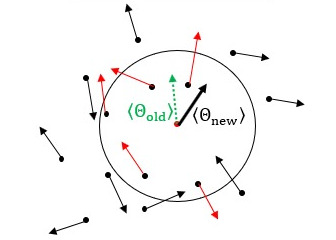
\includegraphics[width=0.3\textwidth]{images/chapter1/particle_direction.jpeg} 
  	%	\caption*{ales.airliquide. \url{https://ales.airliquide.com/our-markets/photovoltaic}. Accessed on the 15.11.2021.}
	%\end{figure}
\end{frame}

\begin{frame}
	\frametitle{1) Motivation and Theory}
	\begin{itemize}
	    \item Updating $\theta_t^i$ using the expression
	    	\begin{equation}
	        	\theta_{t + \Delta t}^i = \langle \theta_t^j \rangle_{|r_i - r_j| < R} + \sqrt{2 D_\mathrm{rot} \Delta t} \cdot \eta_t,
	    	\end{equation} \noindent 
	    with $D_\mathrm{rot}$ as rotational diffusion coefficient and $\eta_t$ as Gaussian noise  
	    \item $\langle \theta_t^j \rangle_{|r_i - r_j| < R}$ describes an average direction obtained via    
	    	\begin{equation}
	        	\langle \theta_t^j \rangle_{|r_i - r_j| < R} = \arctan{\left(\frac{\langle \sin{(\theta_t^j)} \rangle_{|r_i - r_j| < R}}{\langle \cos{(\theta_t^j)} \rangle_{|r_i - r_j| < R}}\right)}
		    \end{equation}
	\end{itemize}
	\begin{figure}[H]
  		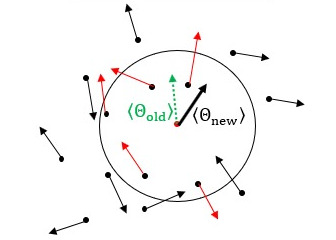
\includegraphics[width=0.3\textwidth]{images/chapter1/particle_direction.jpeg} 
	\end{figure}
\end{frame}

\begin{frame}
	\frametitle{1) Motivation and Theory}
	\textbf{Order Parameter.}
	\begin{itemize}
		\item To study phase transitions we analyse the order parameter $v_\mathrm{a}$
	
			\begin{equation}
	    		v_\mathrm{a} = \frac{1}{N v} \cdot \left| \sum_i^N \mathbf{v}^i \right| \in \left[0,1\right]
			\end{equation}
		\item Order parameter $v_\mathrm{a}$ inhibits (all) physics of the model
	\end{itemize}
\end{frame}